\section{Plan de Proyecto}
\label{sec:planificacion}
\subsection{Iteraciones}
Las iteraciones tienen una duración aproximada de 3 semanas (15 días hábiles). Teniendo en cuenta que los recursos asignados son 4 arquitectos de software/programadores trabajando de modo part-time (6 horas), se estiman unas 360hrs. aproximadas por iteración.

Nuestra decisión sobre la conformación de las iteraciones -en cuanto a los casos de uso- se rigió por varios factores: 
\begin{itemize}
\item Se tuvieron en cuenta las necesidades extraídas del QAW con los stakeholders
\item Se trató de agrupar a los casos de uso por su temática, prefiriendo en caso de ser posible juntar dentro de una misma iteración los casos de uso que se relacionan con funcionalidades similares.
\item Otro factor que se tuvo en cuenta a la hora de definir el orden de las iteraciones, fueron los riesgos detectados y analizados en \refcompleta{sec:riesgos}.
\item También se consideró la prioridad de la funcionalidades referidas en los casos de uso, intentando en lo posible desarrollar antes las más importantes para el negocio.
\end{itemize}

La primera iteración quedó expresamente definida por el QAW y el análisis de riesgo, factores a los que se les dio mayor prioridad. 
Del análisis de riesgo, y dado el factor prioritario que tiene la disponibilidad del sistema, se extrajo que la parte más conflictiva ocurre a la hora de transmitir los desafíos (especialmente para los eventos globales), así como al mostrar correctamente las simulaciones.

El siguiente punto en cuanto a nivel de riesgo, fue lo concerniente a la seguridad, integridad y transparencia de la transmisión de los datos de pago y movimientos de dinero, y las transmisiones de datos usadas para definir los resultados de los partidos de la realidad y minuto a minuto de las simulaciones. Decidimos encarar esto en la segunda iteración del proyecto.

Otro foco de preocupación y de vital importancia para el proyecto, es su alcance y monetización. Por esa razón, se decidió trabajar en lo que respecta a las publicidades del sitio, simulaciones y transmisiones (y el uso de los datos de comportamiento de usuarios), además de la regionalización del sistema (con todas las reglas y restricciones que eso conlleva) en la tercer iteración.

El manejo administrativo de las cuentas de los usuarios, y el aspecto \emph{social} (chat, utilización de las opiniones vertidas en redes sociales, etc.), consideradas cuestiones de menor complejidad, se decidieron enfrentar en la cuarta iteración.

Decidimos dedicarnos en la quinta iteración a todo lo referido a los desafíos, su creación, configuración, definición de reglas y de los premios. En la sexta iteración, nos encargaremos de lo que concierne a los rankings de los jugadores globales, regionales, etc. Como los casos de uso de estas dos iteraciones tienen un menor riesgo y complejidad que los anteriores, consideramos que estas dos fases son de construcción, ya que se trabajará bastante en lo implementativo y poco en el análisis/diseño.



\subsubsection{I01 - Primera Iteración (Elaboración)}
\begin{itemize}
\item (CU19) Mostrando detalle minuto a minuto de la simulación
\item (CU2)  Obteniendo datos en tiempo real
\item (CU21) Mostrando simulación gráfica
\item (CU22) Observando la transmisión de un partido de liga
%\item CU15) Mostrando desarrollo (log o streaming) de desafío} (sistema -> usuario)
\end{itemize}

\subsubsection{I02 - Segunda iteración (Elaboración)} 
\begin{itemize}
\item (CU9) Creando cuenta de usuario
\item (CU10) Actualizando datos de medios de pago
\item (CU34) Auditando movimientos de dinero
\item (CU33) Consultando estado de cuenta y movimientos de usuario
\item (CU35) Auditando simulaciones
\item (CU8) Apostando
%\item CU43) Logueando movimientos de dinero}: (depende de lo que diga Javi)
\end{itemize}


\subsubsection{I03 - Tercera Iteración (Elaboración)}
\begin{itemize}
\item (CU36) Definiendo restricciones por zona
\item (CU25) Definiendo regiones de la plataforma
\item (CU18) Definiendo reglas de simulación
\item (CU38) Configurando publicidad y ads en transmisiones
\item (CU16) Configurando publicidad en el sitio y simulaciones
\item (CU17) Acceder a datos de preferencia/comportamiento de usuarios
%\item (CU44) Mostrando publicidad en la simulación} - ¿es algo que se hace al generar la simulación,  puede ser luego?
%\item (CU37) Configurando publicidades en simulaciones y en el sitio}:  (representante de empresas (?))
%\item (CU39) Consultando datos de usuario}: (representantes de empresas(?))
\end{itemize}


\subsubsection{I04 - Cuarta Iteración (Elaboración)}
\begin{itemize}
\item (CU6) Participando del chat general
\item (CU7) Participando de chat privado
\item (CU12) Consultando cuenta de usuario
\item (CU41) Desactivando cuenta
\item (CU42) Reactivando cuenta
\item (CU23) Recolectando opiniones de redes sociales y chats
\item (CU24) Definiendo impacto de opiniones
%4- consultando datos de jugadores /técnicos /equipos (participante)
\end{itemize}

\subsubsection{I05 - Quinta Iteración (Construcción)}
\begin{itemize}
\item (CU1) Eligiendo liga para competir
\item (CU3) Definiendo reglas de desafío
\item (CU4) Creando desafío
\item (CU5) Aceptando desafío
\item (CU14) Consultando estado (cuenta regresiva, participantes, posiciones) del desafío
\item (CU13) Definiendo premios
\end{itemize}

\subsubsection{I06 - Sexta Iteración (Construcción)}
\begin{itemize}
\item (CU28) Consultando dashboard regional o global
\item (CU29) Consultando ranking de jugadores
\item (CU32) Reiniciando el ranking de jugadores
\item (CU26) Definiendo desafíos interzonales
\item (CU31) Configurando visibilidad de los desafíos
%6 -  definiendo reglas de puntajes (administrador)
\end{itemize}


\subsection{Primera iteración (I01) en detalle}
\label{subsec:primeraiteracion}
En esta sección se realiza un detalle de las tareas que se consideran necesarias realizar en la primer iteración, junto a las horas hombres esperadas. Dado que ya se realizó un reconocimiento, priorización, y estimación de tiempo de los casos de uso, además del análisis de riesgo, no serán tareas prioritarias ni de mucha intensidad en esta etapa, sino que se utilizarán para poder corregir detalles de las futuras iteraciones.

Algunas de las tareas (por ejemplo I01T01, I01T02, I01T03) que no se corresponden directamente con un caso de uso, tienen como objetivo la mitigación de los riesgos analizados (\refcompleta{sec:riesgos}).

\begin{itemize}
\item \underline{I01T01} - Reunión semanal breve con stakeholders para asegurarse que los requerimientos estén actualizados: \textbf{10hs}.
  \begin{itemize}
    \item \underline{I01T01ST01} - Reunión la primer semana: 4hs.
    \item \underline{I01T01ST02} - Reunión la segunda semana: 3hs.
    \item \underline{I01T01ST03} - Reunión la tercer semana: 3hs.
  \end{itemize}
\hfill

\item \underline{I01T02} - Reunión cada 3 días hábiles del equipo para evitar problemas de comunicación como en el pasado: \textbf{10hs}.
  \begin{itemize}
    \item \underline{I01T02ST01} - Primera reunión: 2hs.
    \item \underline{I01T02ST02} - Segunda reunión: 2hs.
    \item \underline{I01T02ST03} - Tercer reunión: 2hs.
    \item \underline{I01T02ST04} - Cuarta reunión: 2hs.
    \item \underline{I01T02ST05} - Quinta reunión: 2hs.
  \end{itemize}
\hfill

\item \underline{I01T03} - Reunión semanal de consulta con experto en metodología UP: \textbf{8hs}.
  \begin{itemize}
    \item \underline{I01T03ST01} - Reunión la primer semana: 3hs.
    \item \underline{I01T03ST02} - Reunión la segunda semana: 2hs.
    \item \underline{I01T03ST03} - Reunión la tercer semana: 2hs.
  \end{itemize}
\hfill

\item \underline{I01T04} - Identificación y descripción de los atributos de calidad del sistema: \textbf{40hs}.
  \begin{itemize}
    \item \underline{I01T04ST01} - Cotejamiento de los atributos definidos por stakeholders en QAW y relación con los casos de uso definidos: 16hrs.
    \item \underline{I01T04ST02} - Descripción de escenarios de atributos de calidad: 20hs.
    \item \underline{I01T04ST03} - Verificación de la documentación escrita: 4hs.
  \end{itemize}
\hfill
  
\item \underline{I01T05} - Diseño de la arquitectura del sistema: \textbf{60hs}.
  \begin{itemize}
    \item \underline{I01T05ST01} - Analizar los escenarios descritos en I01T04 e identificar drivers de arquitectura: 8hs. 
    \item \underline{I01T05ST02} - Estudiar y elegir patrones arquitectónicos que satisfagan los drivers identificados: 12hs.
    \item \underline{I01T05ST03} - Verificar y refinar los casos de usos y los escenarios: 10hs.
    \item \underline{I01T05ST04} - Iterar: 30hs.
   \end{itemize}
\hfill

\item \underline{I01T06} - Realización de las tareas del (CU2)  Obteniendo datos en tiempo real: \textbf{40hs}.
  \begin{itemize}
    \item \underline{I01T06ST01} - Reunirse con empresas que provean datos en tiempo real de la evolución de los partidos y contratar alguna: 12hs.
    \item \underline{I01T06ST02} - Reunirse con la empresa contratada y obtener documentación técnica sobre la API que proveen: 2hs.
    \item \underline{I01T06ST03} - Investigar la API y analizar qué datos podemos usar como input en nuestro sistema: 6hs.
    \item \underline{I01T06ST04} - Adaptar nuestro sistema para que los desafíos en modo \emph{Liga de fantasía} utilicen los datos obtenidos a través de la api: 10hs.
    \item \underline{I01T06ST05} - Realizar algunos desafíos y verificar que los resultados de los puntajes se condigan con lo que ocurrió en los partidos reales: 6hs.
    \item \underline{I01T06ST06} - Corregir potenciales errores: 4hs.
  \end{itemize}
\hfill

\item \underline{I01T07} - Realización de las tareas del (CU19) Mostrando detalle minuto a minuto de la simulación: \textbf{40hs}.
  \begin{itemize}
    \item \underline{I01T07ST01} - Investigar el log del desarrollo anterior, cómo se genera y la calidad de la salida: 4hs.
    \item \underline{I01T07ST02} - Reunirse con las empresas desarrolladoras de los dos motores gráficos y averiguar qué tipo de entrada necesitan: 6hs.
    \item \underline{I01T07ST03} - Comparar el log actual con el que se necesita y definir qué es lo que falta agregar: 4hs.
    \item \underline{I01T07ST04} - Agregar el detalle necesario al log de salida para cumplir con lo requerido por las empresas: 10hs.
    \item \underline{I01T07ST05} - Ajustar la velocidad de salida del log para que no sea instantánea, sino minuto a minuto, y respete la nueva duración (similar a la de un partido real) de las simulaciones: 5hs.
    \item \underline{I01T07ST06} - Realizar algunas ejecuciones de prueba y obtener logs de salida de ejemplo: 4hs.
    \item \underline{I01T07ST07} - Corroborar con empresas proveedoras que el detalle del log obtenido sea el correcto: 2hs.    
    \item \underline{I01T07ST08} - Corregir potenciales errores: 5hs.
  \end{itemize}
\hfill

\item \underline{I01T08} - Realización de las tareas del (CU21) Mostrando simulación gráfica: \textbf{50hs}.
  \begin{itemize}
    \item \underline{I01T08ST01} - Reunirse con empresa de motor 3D y discutir sobre los requerimientos técnicos para la transmisión de video en dispositivos no soportados por el motor gráfico: 10hs.
    \item \underline{I01T08ST02} - Obtener varios logs minuto a minuto de prueba y utilizarlos como entrada para los distintos motores gráficos. Comparar que el resultado gráfico (según limitaciones de cada motor) de los partidos sea el mismo y no haya diferencias: 20hs.
    \item \underline{I01T08ST03} - Probar los motores en distintos dispositivos y obtener los requerimientos mínimos y recomendados de hardware para poder informar a los participantes: 15hs.
    \item \underline{I01T08ST04} - Escribir documentación sobre los distintos motores, obtener screenshots para poder publicar en el home del producto como ejemplo de jugabilidad: 5hs.
  \end{itemize}
\hfill


\item \underline{I01T09} - Realización de las tareas del (CU22) Observando la transmisión de un partido de liga: \textbf{80hs}.
  \begin{itemize}
    \item \underline{I01T09ST01} - Reunirse con la empresa dueña de los derechos de televisión y la empresa proveedora de infraestructura para definir sus requerimientos, necesidades, y llegar a acuerdos comunes en los puntos álgidos: 15hs.
    \item \underline{I01T09ST02} - Reunirse con la empresa proveedora de infraestructura de redes para definir la arquitectura de hardware a utilizar para el sistema: 10hs.
    \item \underline{I01T09ST03} - Implementar la solución de hardware convenida con la empresa proveedora de infraestructura de redes: 20hs.
    \item \underline{I01T09ST04} - Realizar pruebas internas de transmisión en vivo de eventos con diferentes cargas en los servidores y desde distintas regiones: 15hs.
    \item \underline{I01T09ST05} - Dar feedback a la empresa proveedora de infraestructura y ver, de ser necesario, cómo mejorar el rendimiento: 10hs.
    \item \underline{I01T09ST06} - Mostrarle a la empresa dueña de los derechos de televisión el funcionamiento del sistema y verificar que cumpla con sus requerimientos: 10hs.
  \end{itemize}
\hfill
\end{itemize}
La suma de las tareas para la primer iteración da 338hs. Habiendo calculado una iteración ideal de 360hs. nos da cierto margen como para poder afrontar tareas urgentes o no previstas.

\subsection{Diagrama de Gantt}
  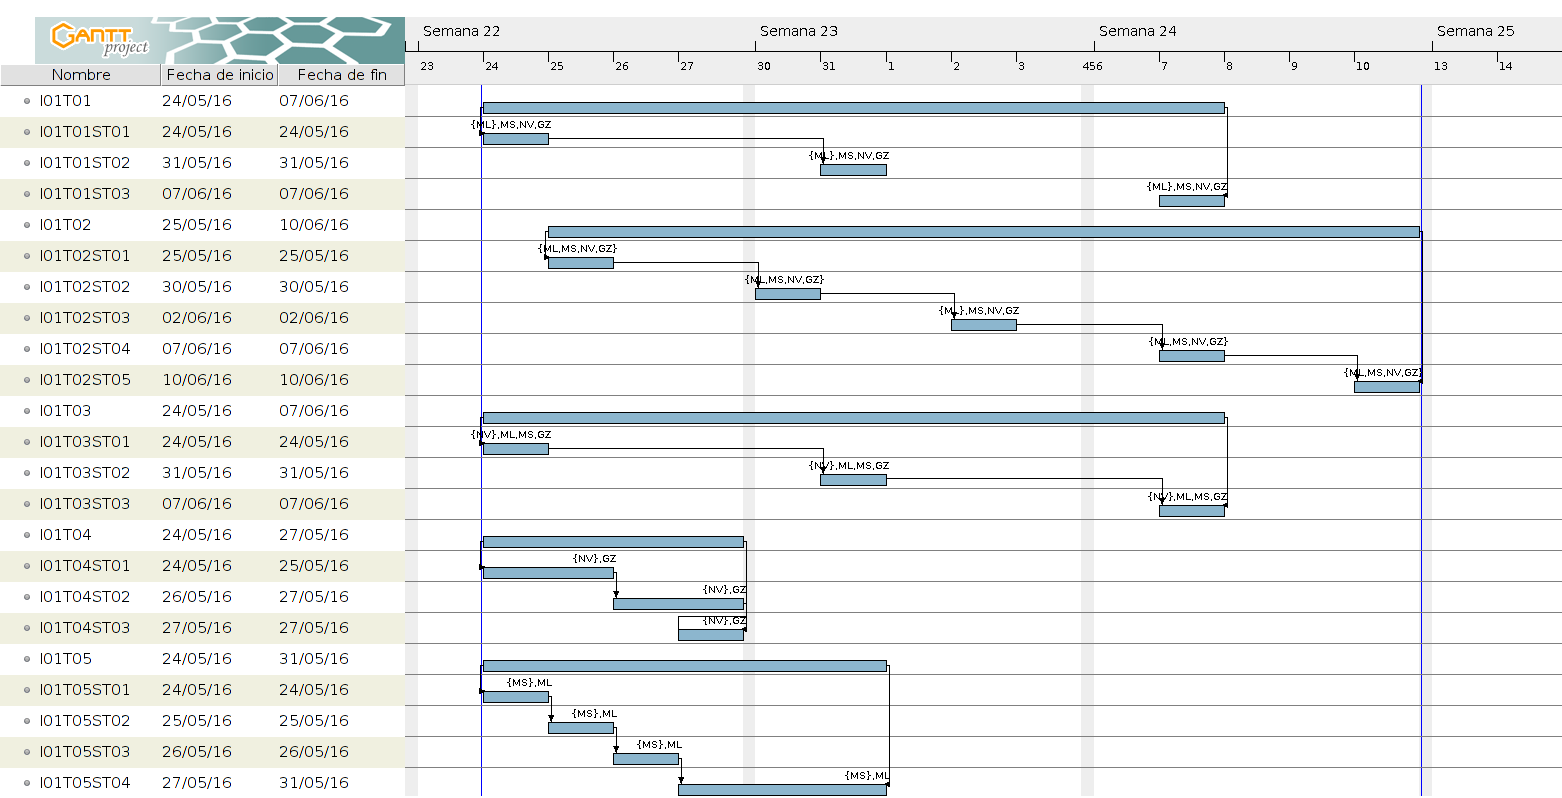
\includegraphics[scale=0.438, angle=90]{images/gantt1.png}
  \newpage
  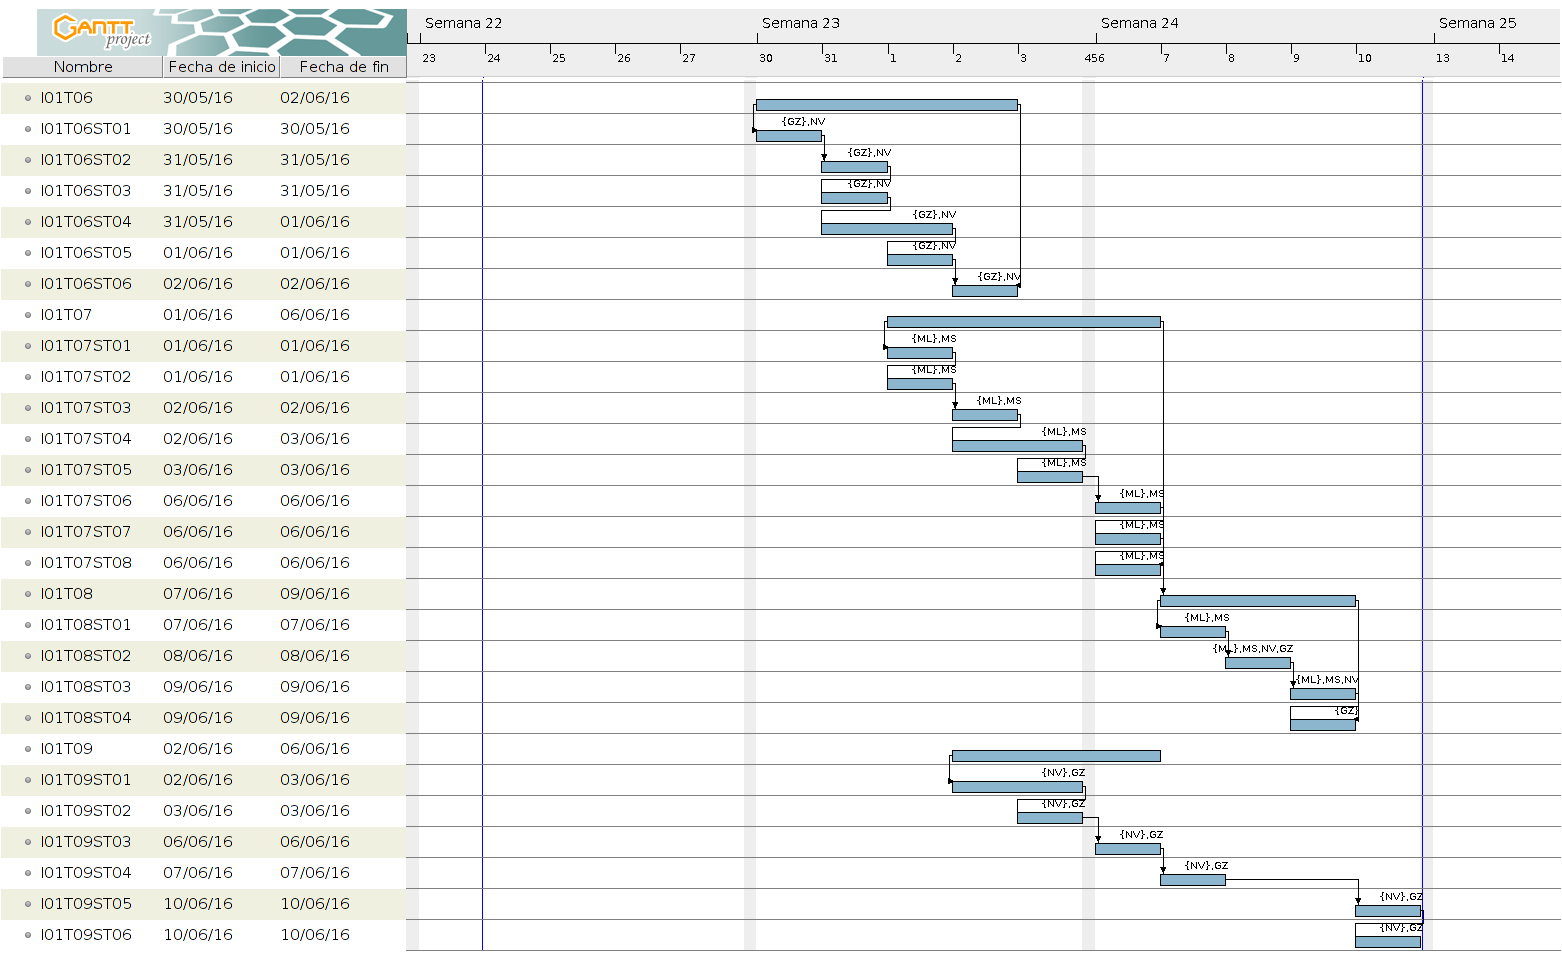
\includegraphics[scale=0.45, angle=90]{images/gantt2.png}

